\section{Memory testing}
\textbf{Выданные параметры:} [fork-vm,zlib-mem-level]
\subsection{zlib}
\nquote{--zlib N}{start  N workers compressing and decompressing random data using zlib. Each worker has two processes,
one that compresses random data and pipes it to another process  that  decompresses  the  data.  This
stressor exercises CPU, cache and memory.}
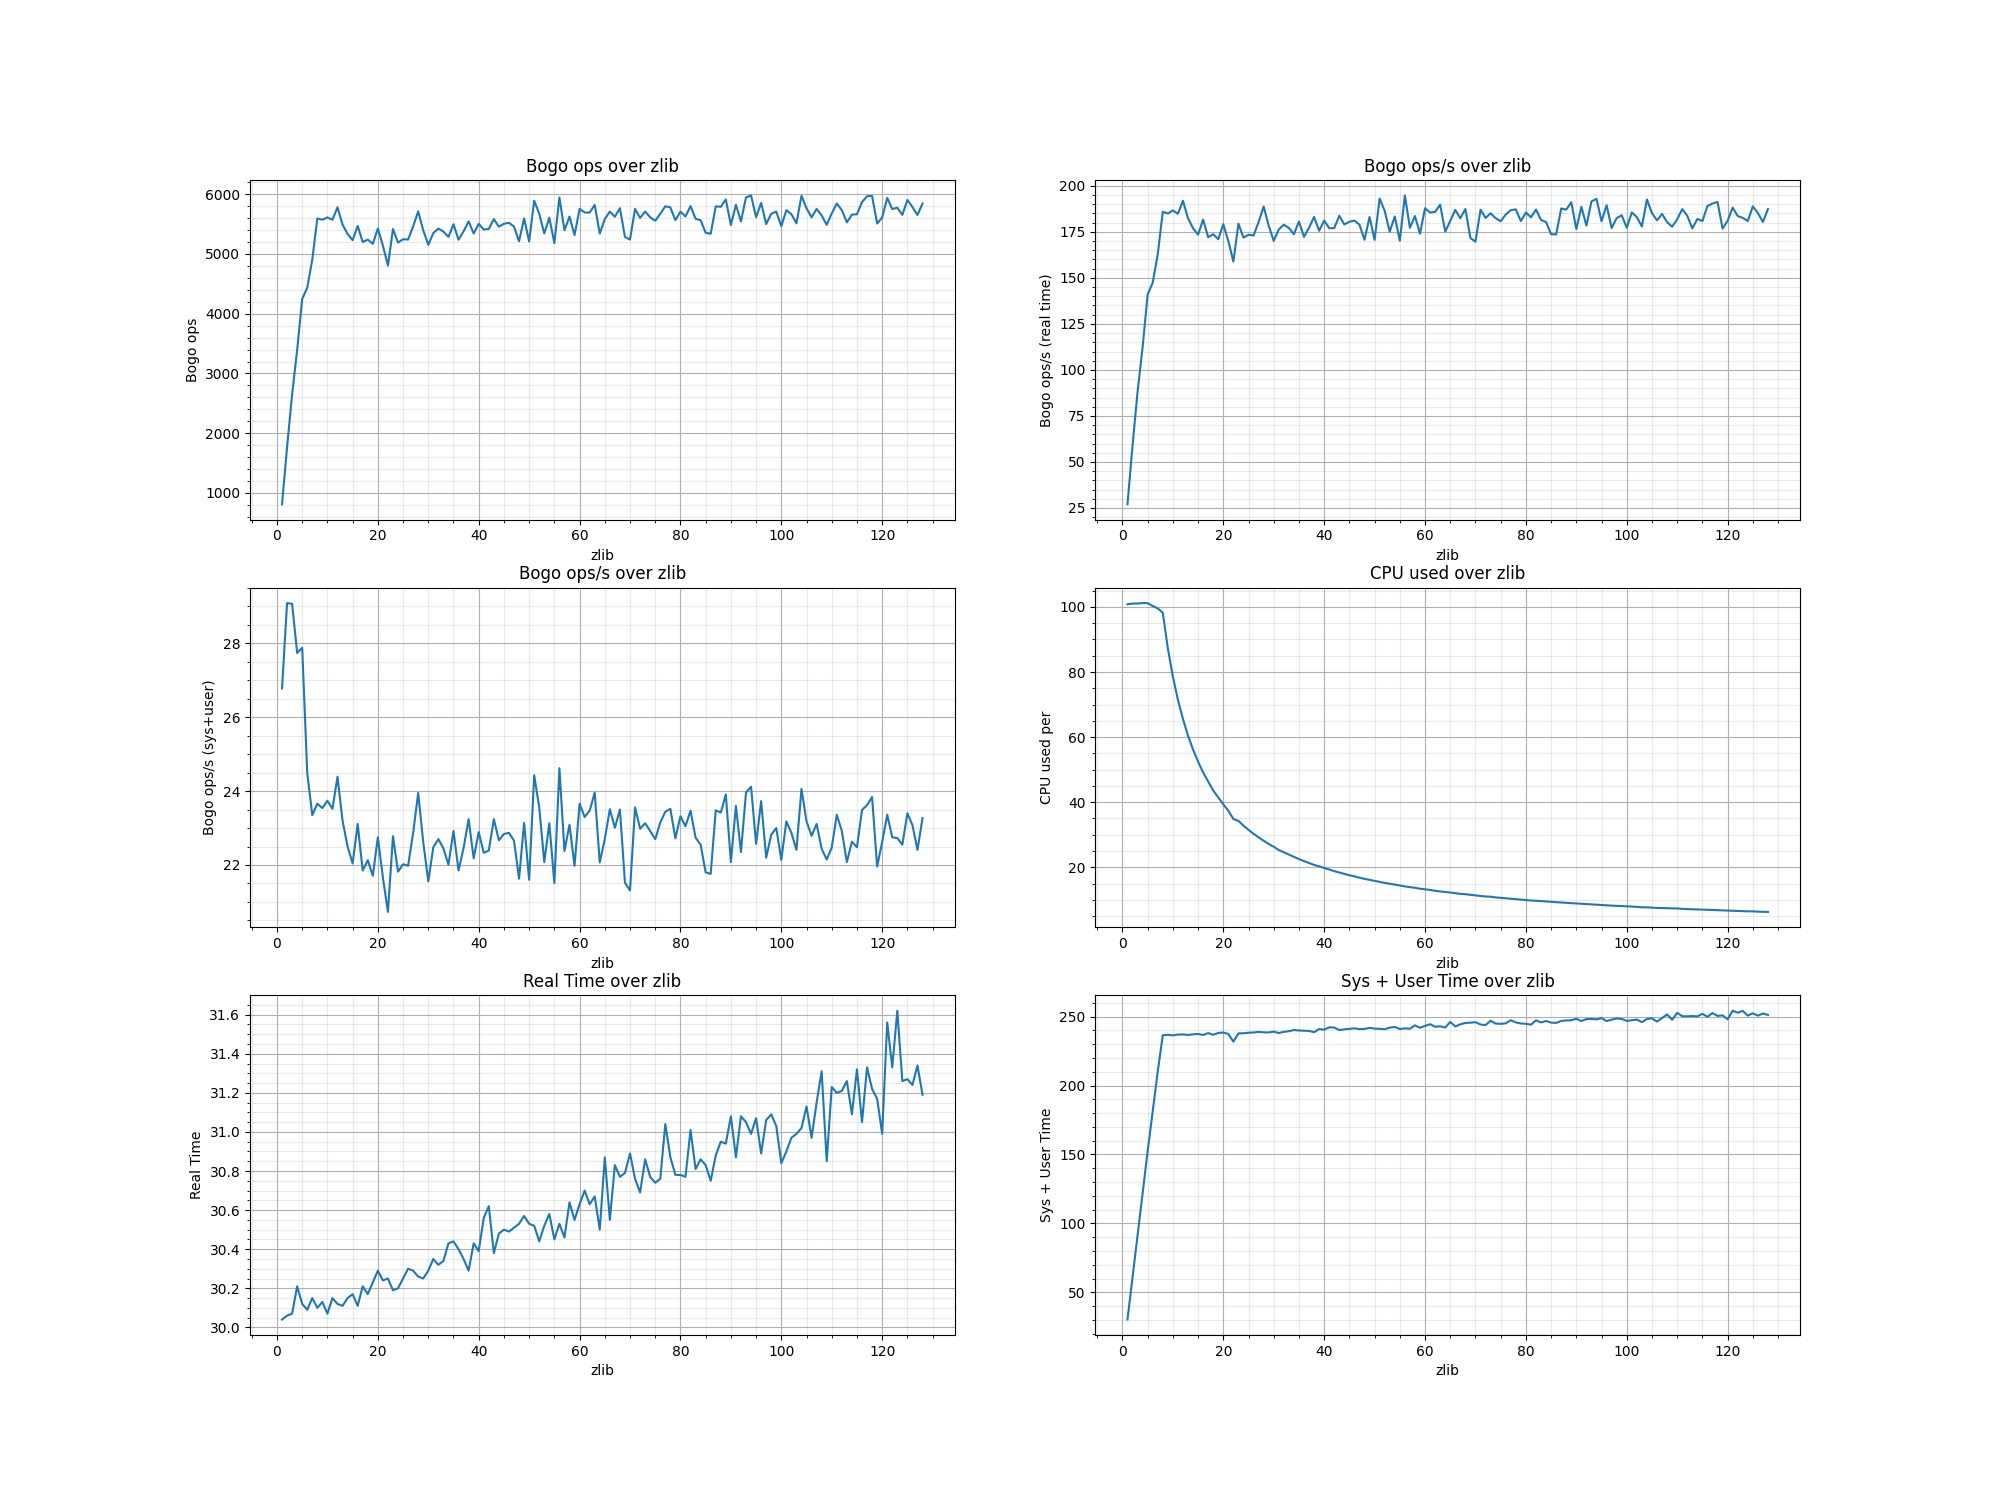
\includegraphics[width=\textwidth]{./memory/image/zlib-bogops.png}
Видим, что 8 воркеров - это оптимальное число.
\subsection{zlib-mem-level}
\nquote{--zlib-mem-level L}{specify the reserved compression state memory for zlib.  Default is 8.
Values:
1 = minimum memory usage
9 = maximum memory usage}
Переберем все значения параметра:
\lstinputlisting[]{memory/scripts/zlib-mem-level-compr.zsh}
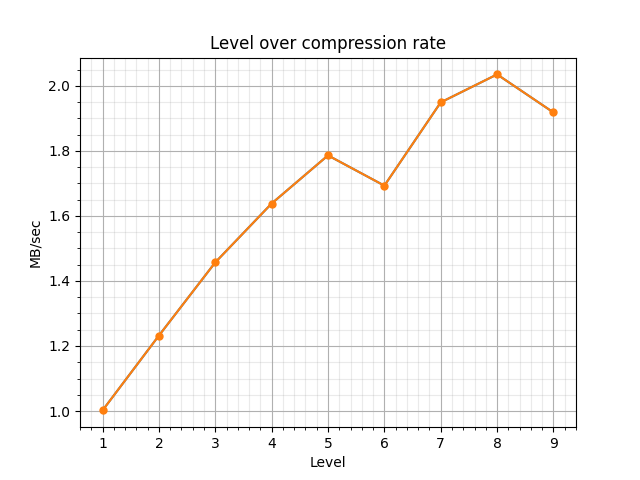
\includegraphics[width=\textwidth]{./memory/image/zsh-mem-level-compr.png}
Видим, что с увеличением уровня увеличивается compression rate достигая максимального значения при 8.\\
Посмотрим на Flamegraph процесса zlib.\\
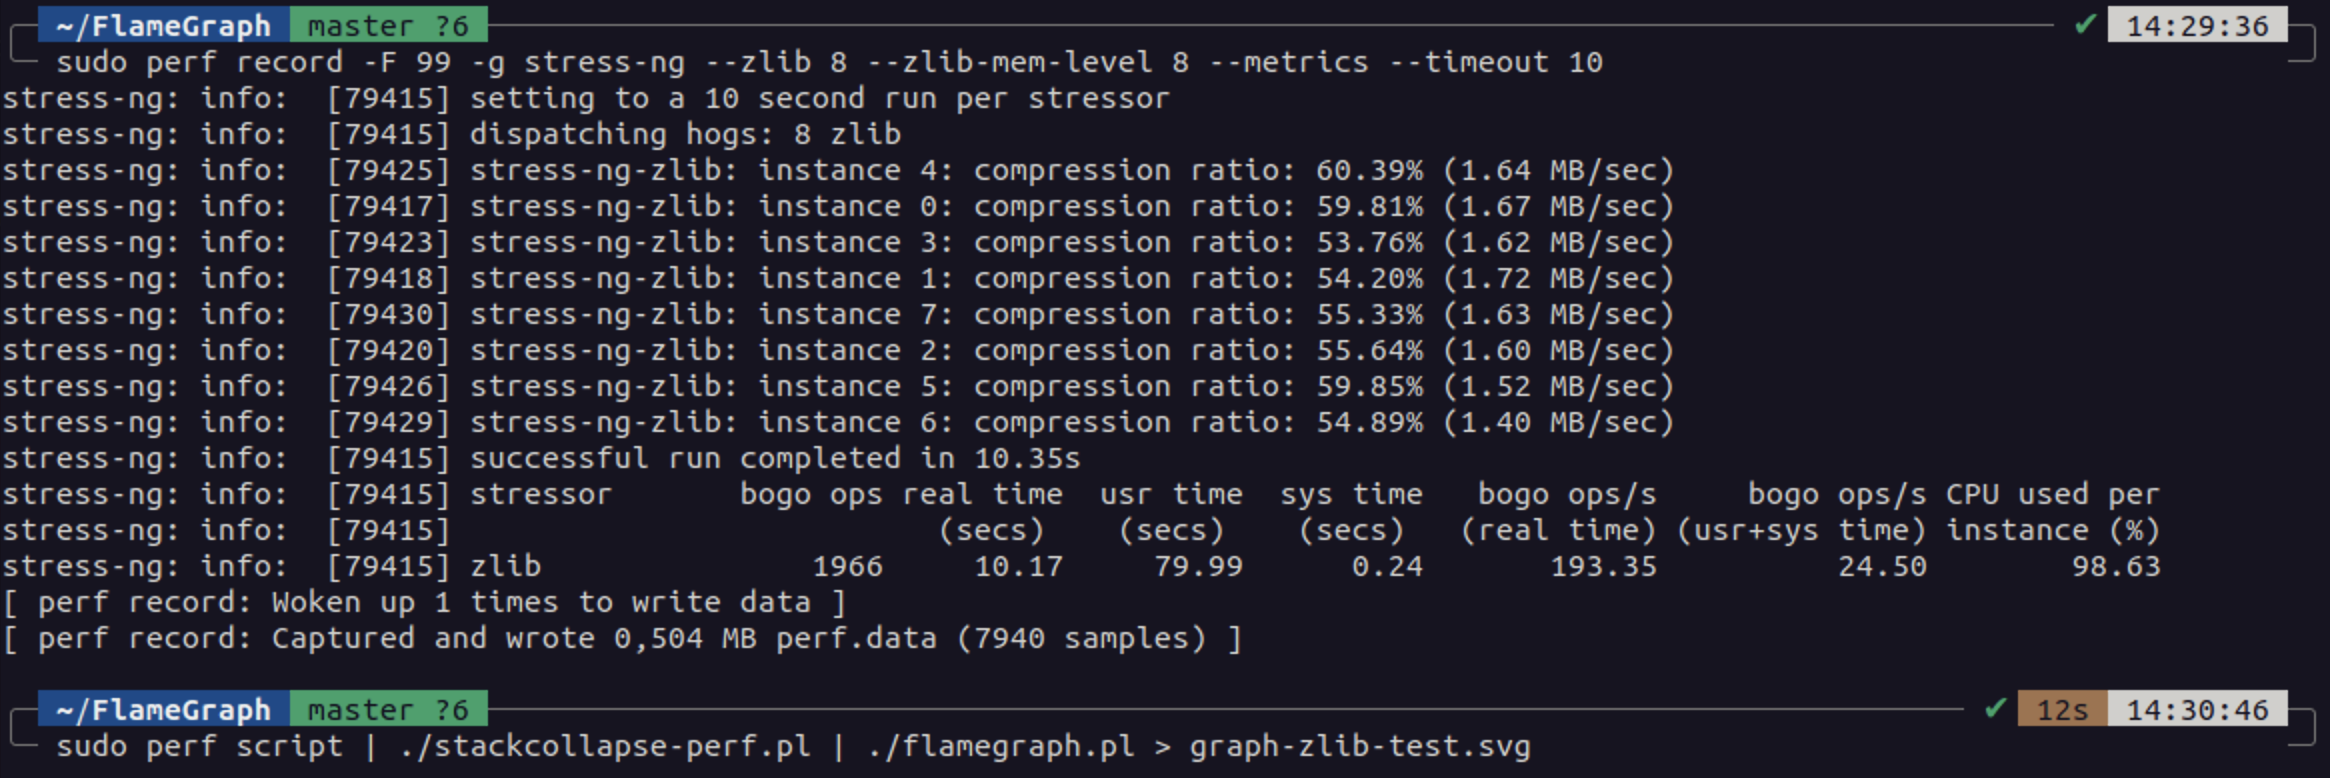
\includegraphics[width=\textwidth]{./memory/image/Flamegraph-script.png}
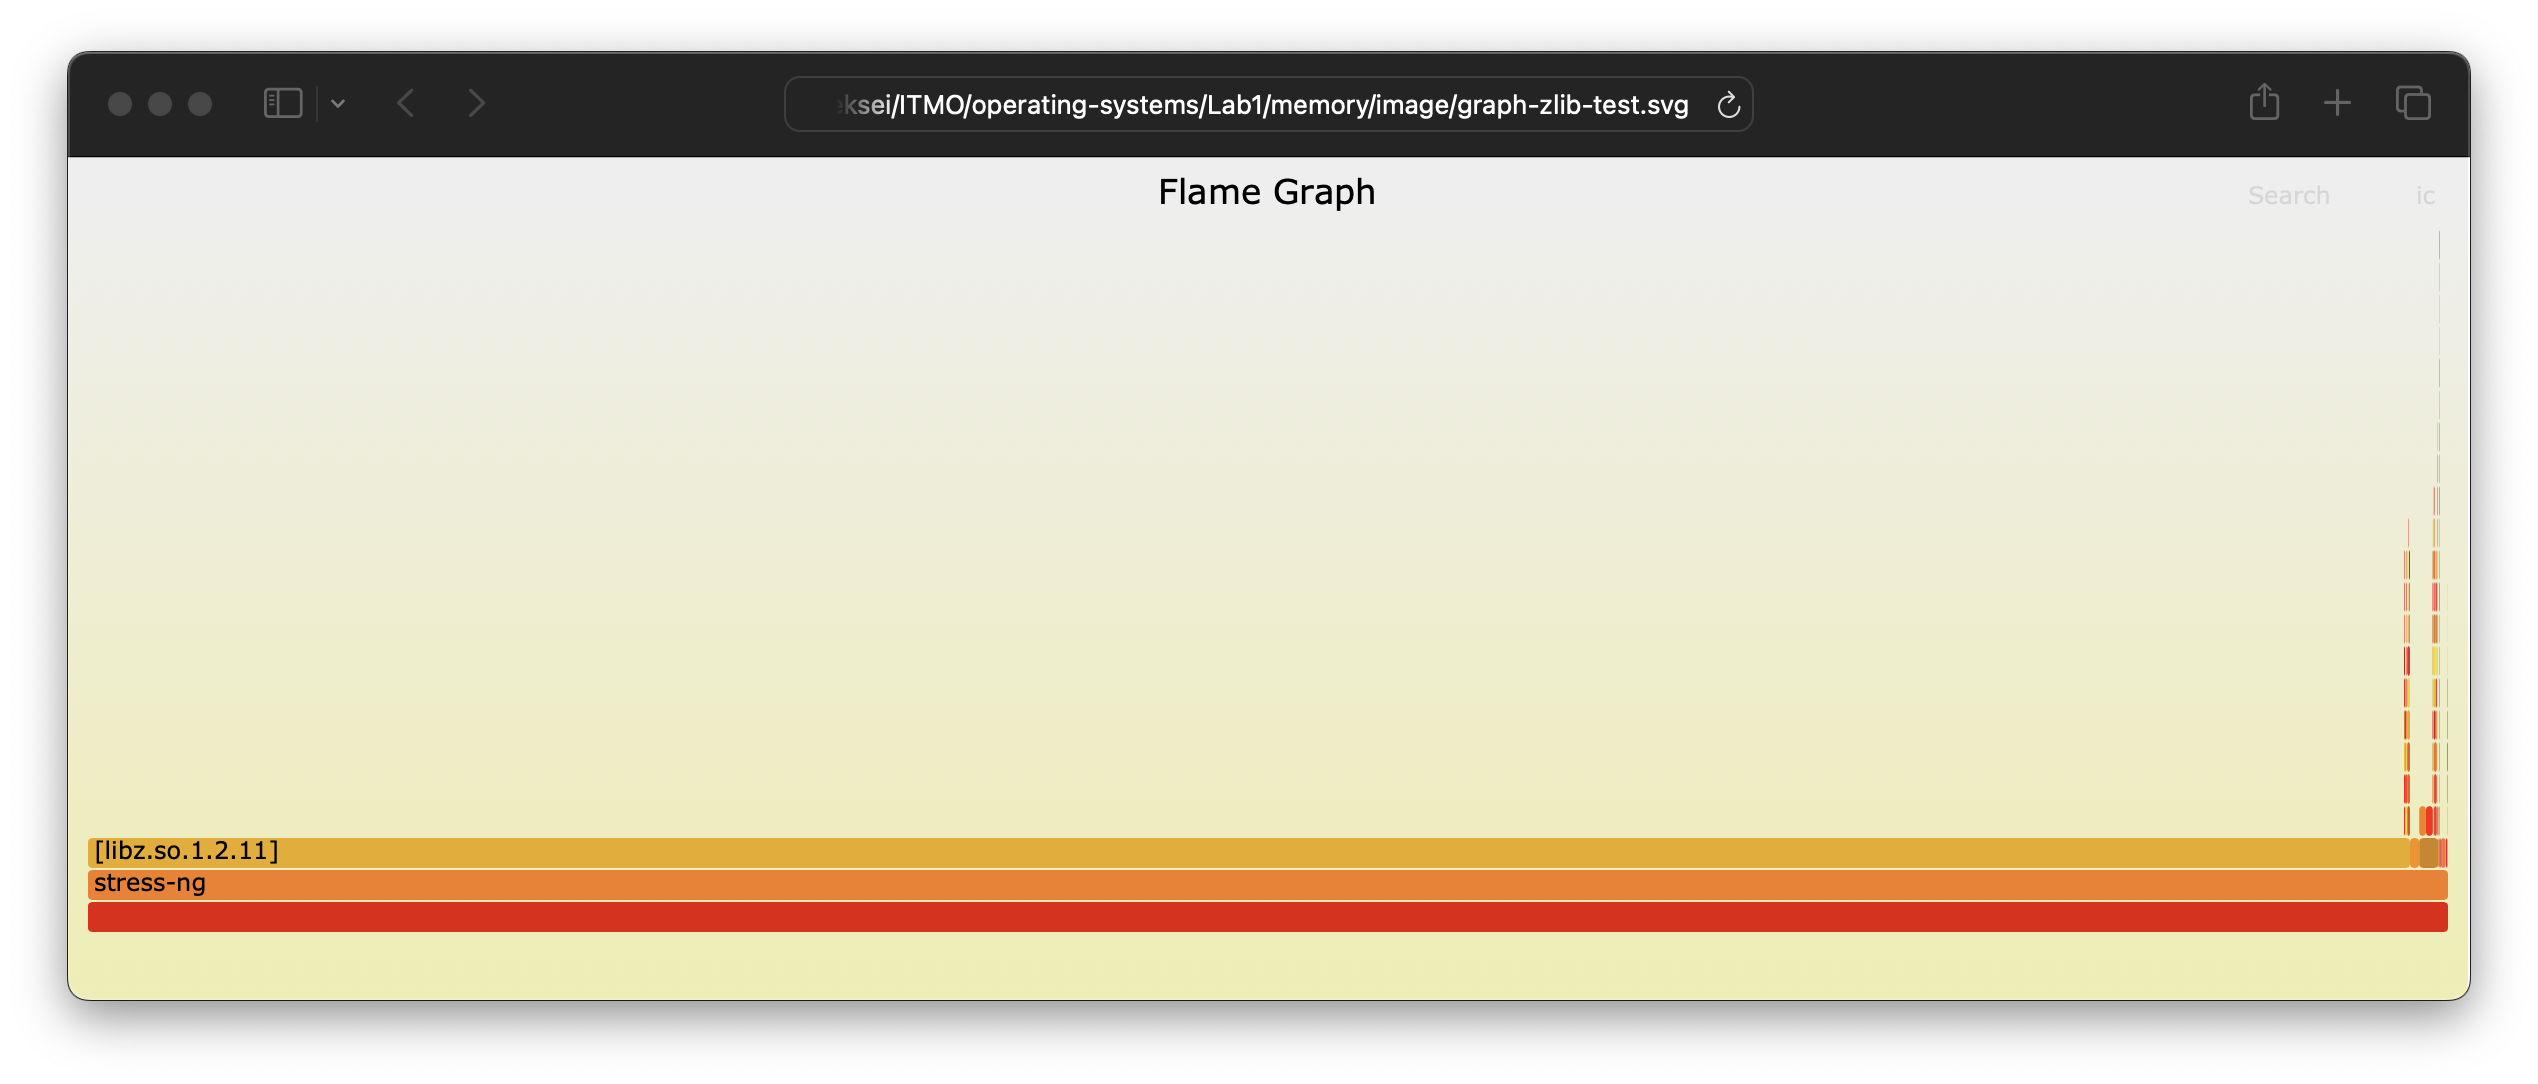
\includegraphics[width=\textwidth]{./memory/image/graph-zlib-test.png}
\subsection{fork-vm}
\nquote{--fork-vm}{enable  detrimental  performance  virtual  memory  advice  using  madvise  on all pages of the forked process. Where possible this will try to set every  page  in  the  new  process  with  using  madvise 
$MADV\_MERGEABLE$, $MADV\_WILLNEED$, $MADV\_HUGEPAGE$ and $MADV\_RANDOM$ flags. Linux only.}
\nquote{MADV\_MERGEABLE}{Включите объединение одинаковых страниц ядра (KSM) для страниц в диапазоне, указанном addr и длиной.  Ядро регулярно сканирует те области пользовательской памяти, которые были помечены как доступные для объединения, в поисках страниц с идентичным содержимым.  Они заменяются одной страницей, защищенной от записи (которая автоматически копируется, если процесс позже захочет обновить содержимое страницы).  KSM объединяет только частные анонимные страницы (см. mmap(2)).
Функция KSM предназначена для приложений, которые генерируют множество экземпляров одних и тех же данных (например, систем виртуализации, таких как KVM). Он может потреблять много вычислительной мощности; используйте его с осторожностью.}
\nquote{MADV\_WILLNEED}{Данные будут использоваться повторно (кэширование желательно)}
\nquote{MADV\_HUGEPAGE}{Включить функцию Transparent Huge Pages (THP) для страниц в диапазоне, заданном addr и length.  В настоящее время Transparent Huge Pages работает только с частными анонимными страницами (см. mmap(2)).  Ядро будет регулярно сканировать области, помеченные как кандидаты на огромные страницы, чтобы заменить их на огромные страницы.   Ядро также будет выделять огромные страницы напрямую, если область естественным образом выровнена по размеру огромной страницы (см. posix\_memalign(2)). Эта функция предназначена в первую очередь для приложений, использующих большие отображения данных и обращающихся к большим областям памяти за один раз (например, системы виртуализации, такие как QEMU).  Это может привести к нерациональному расходованию памяти (например, отображение размером 2 МБ, при котором доступ осуществляется только к одному байту, приведет к использованию 2 МБ проводной памяти вместо одной страницы размером 4 КБ).}
\nquote{MADV\_RANDOM}{Доступ к данным в файле будет произвольным}
Посмотрим, как изменяется количество свободных страниц виртуальной памяти с помощью \textit{vmstat} при включенной и выключенной опции \textit{fork-vm};\\
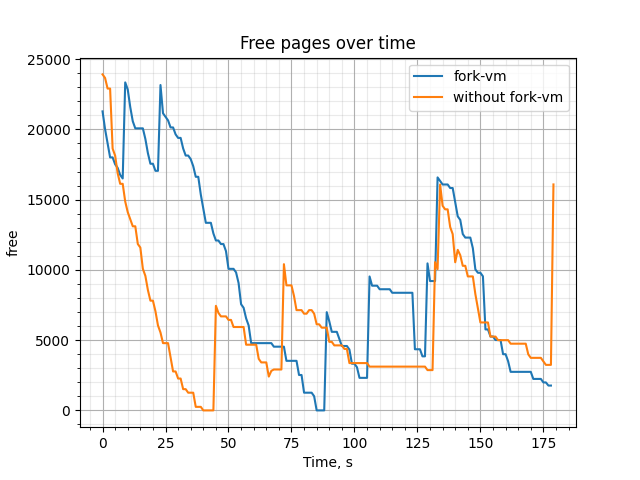
\includegraphics[width=\textwidth]{./memory/image/fork-vm.png}
Видим, что особого влияния на количество свободных страниц виртуальной памяти нет.\\
